\begin{figure}
	\centering
	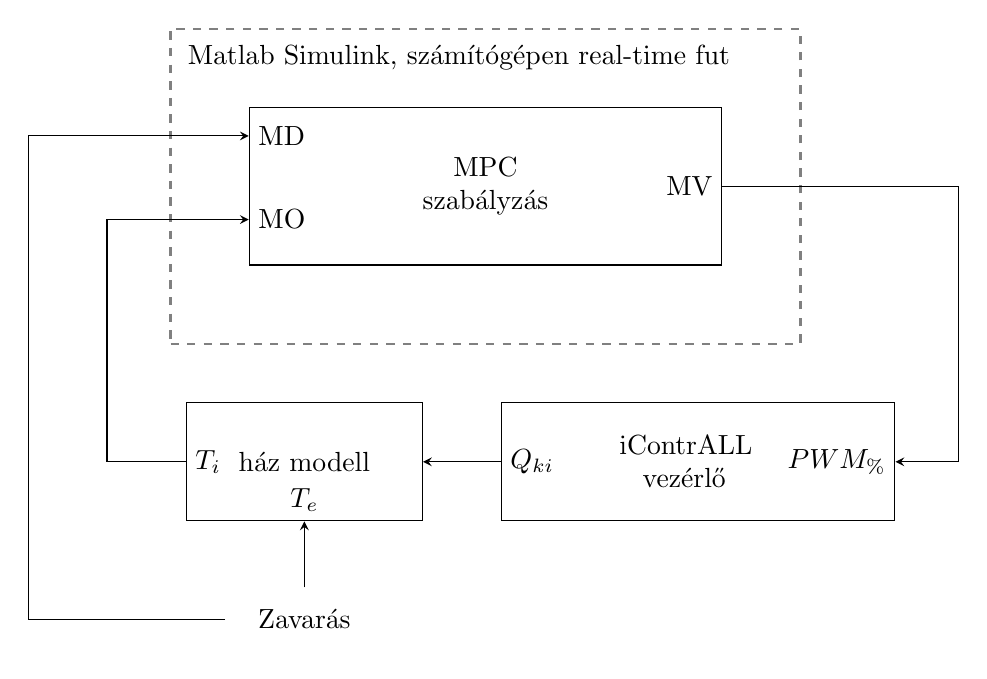
\begin{tikzpicture}[>=stealth,
  		%inner/.style={draw,fill=blue!5,thick,inner sep=3pt,minimum width=8em},
		%outer/.style={draw=gray,dashed,fill=green!1,thick,inner sep=5pt}
		outer/.style={draw=gray,dashed,thick,inner sep=5pt}
		]
	\node[rectangle, minimum height=0.8cm,minimum width=2cm] (ghostDist) at (0,-2) {Zavarás};
	
	% Szabályzási kör elemei
	% ----------------------
	
		% Szabályzó
		\node[draw,rectangle, minimum height=2cm,minimum width=6cm] (MPC) at (2.3,3.5) {\parbox{2cm}{\centering MPC szabályzás}};		

		% Fűtési rendszer
		\node[draw,rectangle, minimum height=1.5cm,minimum width=5cm] (Heat) at (5,0) {\parbox{2cm}{\centering iContrALL~~~~ \\ vezérlő~~~~}};
	
		% Ház
		\node[draw,rectangle, minimum height=1.5cm,minimum width=3cm] (House) at (0,0) {ház modell};
		\draw[->] (ghostDist.90) --  (House.270) node[above]{$T_e$}; 
		
	
	% Kiegészítő cuccok
	% ----------------------
	
	% Keret - Matlab
	\node[draw,outer,rectangle, minimum height=4cm,minimum width=8cm,
	label={[label distance=-0.1cm, anchor=north]100:Matlab Simulink, számítógépen real-time fut}] (keret) at (2.3,3.5) {};
	
	% Zavarás a modellbemenetre
	\draw[->] (ghostDist.180) -| ++(-2.5,0)  |-  (MPC.168) node[right]{MD} ;
	
	%\draw[->] (ctr.191) node[right]{${u_{2}}$} -| ++(-1.7,1.3)|-  (Numeric.172) node[right]{$\alpha_{floor}$};  %node[above left]{$\alpha_{radiator}$}; 
	
	% mért változó
	\draw[->] (House.180) node[right]{${T_{i}}$}-| ++(-1,0.8)  |-  (MPC.188) node[right]{MO} ;
	
	%\draw[->] (d.0) node[left]{heat [W]} ->  ++(3,0) ->  (house.180);
	\draw [->] (MPC.0) node[left]{MV} -| ++(3,-2.5)  |- (Heat.0) node[left]{${PWM_{\%}}$}; %++(1.5cm,0) -- (2cm,0pt) -- (2.5cm,10pt);
	
	\draw[->] (Heat.180)  node[right]{$Q_{ki}$} -- (House.0) ;
	%\draw[->] (d.20) -| ++(1,-1) |- (y.350);
	
	%\path 
	%(d.150)	 edge[<->] 	node[anchor=north,above]{valvePercent}	(y.270);
	
	% Lehetséges label beállítások:
		%label={[blue,yshift=0.3cm]above:Z}]
	
	\end{tikzpicture}

	\caption{A szimulációban szereplő elemek kapcsolata}
	\label{fig_realtimesimulink}
\end{figure}

%\begin{tikzpicture}[>=stealth,remember picture]
%\node[draw,rectangle,inner sep=0.5cm] (y) at (0,0) {$A$};
%\node[draw] (d) at (0,2) {%
%%	\begin{tikzpicture}[remember picture]
%%	\matrix [matrix of math nodes] (mat)
%%	{
%%		B & \phantom{C}   \\
%%		\phantom{B} & C \\
%%	};
%%	\end{tikzpicture}
%%};
%%\draw[->,shorten >= 6pt] (y.west) -| ++(-1,1) |- (mat-1-1);
%%\draw[->,shorten >= 6pt] (y.west) -| ++(-0.8,1) |- (mat-2-1);
%%\draw[->] ($(mat-2-2)+(14pt,0)$) -| ++(0.8,-1) |- (y.east);
%%\draw[->] ($(mat-1-2)+(14pt,0)$) -| ++(1,-1) |- (y.east);
%\end{tikzpicture}

